\chapter[Introdução à edição brasileira]{Introdução à edição brasileira \subtitulo{Vilna no Brasil}}
\hedramarkboth{Introdução}{}

\begin{flushright}
\textsc{laimonas briedis}
\end{flushright}

\setlength{\epigraphwidth}{.65\textwidth}
\begin{epigraphs} 
\qitem{Mas a saudade é isto mesmo; é o passar e repassar das memórias
antigas.}{\textit{Dom Casmurro}, \textsc{machado de assis}}

\medskip

\qitem{Ó, Lituânia, pátria minha, mordida de serpente no meu coração,\\
Cegonhas, adejando em minha memória por sobre sua floresta negra,\\
Como sinais cabalistas, douram as bordas\\
Onde seus abetos farfalham nas margens do Viliya}{\textsc{abraham sutzkever}}
\end{epigraphs}

%\section*{A cartografia medieval de Angelino}

\noindent{}Brasil e Lituânia formam um encontro inaudito --- tão distantes um do
outro, geográfica e culturalmente, quase em polos opostos. O Brasil é um
sub"-continente, colosso de oportunidades aparentemente ilimitadas,
comparado pela letra do hino nacional a um sonho intenso, talvez mais
promissor que real, aclamado como um reino dourado de qualificações
paradisíacas. A Lituânia, por sua vez, é um pontinho no mapa da Europa:
um território mínimo e compacto, apequenado tanto em tamanho como em
população por seus vários vizinhos. 

Só um pouco maior que o estado da
Paraíba, a Lituânia corresponde a menos de um por cento da área total do
Brasil. Pode"-se atravessar facilmente o país de carro, desde a fronteira
letã ao norte até a fronteira polonesa, numa questão de quatro ou cinco
horas; e, desde a altitude de cruzeiro de uma aeronave, todo o
território do Mar Báltico a oeste até os confins invisíveis com a
Bielorrússia a leste pode ser vislumbrado num único instante.

Observando"-a, a Lituânia é elementar: horizontal e presa à terra.
Ganhar o país a partir do oeste pode ser descrito mais precisamente como
um escurecimento da paisagem, com campos aráveis que gradualmente se
transformam ``em pastos, pastos em florestas, florestas em cursos de
água, água em vapores e pântanos cheios de touceiras. Cada alteração é
marcada por uma mudança simples e limitada de cores.''\footnote{Dan Jacobson, \textit{Heshel's Kingdom}. Londres: Penguin Books, 1998, p. 109.}

Contudo, se o Brasil pode ser resumido como detentor de uma incomparável
panóplia de matizes geográficas e diversidade humana, a Lituânia, por
seu lado, com suas dimensões de bolso, ostenta a marca de uma história
digna de um império. É difícil sintetizar a maior parte de seu passado,
pois, em diversas passagens, ele pertence à história de outros
países e à memória de diferentes povos. Como resultado, a compleição da
Lituânia tem o caráter do camaleão --- ora visível, ora invisível. A
antiga Lituânia já tinha mais ou menos se desintegrado à época em que o
Brasil se destacou de Portugal em 1822. Quase cem anos depois --- mais
exatamente em 1918 --- a independência da Lituânia foi reconstituída,
porém sob circunstâncias políticas e culturais completamente distintas,
que desafiavam a lógica do passado. 

Nos cálculos dos anos, o Brasil é
bem mais velho que a Lituânia. No todo, a Lituânia contemporânea é,
portanto, uma migalha da impressão que deixou na história; comparável,
talvez, a uma lasca de âmbar, resto fragmentário da antiga floresta
esporadicamente presente no litoral lituano do Mar Báltico. O âmbar é
naturalmente escuro, mas se torna luzidio quando exposto ao sol. Do
mesmo modo como a Lituânia que, embora sempre encoberta por sombras nos
relatos históricos da Europa, cintila assim que é removida de seu ponto
cego. Obviamente, os países não são meras cronologias e efemérides, mas
também personalidades que só podem ser amparadas pela imaginação; e, por
mais estranho que pareça, a Lituânia e o Brasil se encontraram pela
primeira vez graças a um julgamento equivocado.

O nome e a localização de ambos os países surgem, pela primeira vez, e
num mesmo mapa, no ano de 1325 (alguns estudiosos apontam 1330),
concebido pela mente de um cartógrafo medieval de nome quase
querubínico: Angelino. Pouco se sabe a respeito desse Angelino, nem
mesmo o seu sobrenome é conhecido ao certo (há quem diga que fosse
Dulcert, ou Dalorto), supõe"-se porém que teria nascido na Ligúria e
aprendido o ofício da cartografia na grande cidade portuária de Gênova.
Mas --- e isso é certo --- ele desenvolveu suas habilidades confeccionando
cartas náuticas na ilha de Maiorca, que, naquela altura, pertencia à
Coroa de Aragão. 

Conhecidas como \textit{portolanos}, as cartas náuticas
incitavam os sonhos dos marinheiros, delineando litorais como se fossem
fibras, que parecem mais corredores aéreos do que pontes ligando terra
firme. Mesmo que não houvesse sido ele próprio marinheiro, Angelino era
no mínimo uma progenitura do Mar Mediterrâneo, capaz de retratar o mundo
com o entusiasmo de quem cruza mares, prevendo costas distantes através
de tormentas, noites estreladas, nevoeiro e tudo o mais. 

Quando o olhar
de Angelino atingiu o norte do Oceano Atlântico e o Mar Báltico, ele
encontrou uma grande carência de precisão cartográfica. O mar para além
da linha costeira é turvo, e a terra firme parece distante,
generalizada. Entretanto, baseando"-se no máximo de seu conhecimento,
Angelino localizou o Brasil num naco de terra quase circular, não muito
distante da costa meridional da Irlanda, numa latitude de cerca de 51°N.
Deu inclusive a essa ilha a seguinte legenda: \textit{Insula de montonis
sive de brazile}, sendo que \textit{montonis} tem sido alternadamente
interpretado como ovelhas ou montanhas.

De todo modo, a palavra \textit{brazile} (ou \textit{Brasil}) muito
provavelmente se origina de uma tinta cujo nome deriva de sua intensa
coloração vermelha. Sabe"-se que a tinta \textit{brazile} é sobretudo
extraída do campeche, conhecido em geral como pau"-brasil. Contudo, na
Antiguidade e na Idade Média, a tinta \textit{brazile} era importada do
Oriente Médio para a Europa. Mais de um século antes do início da
colonização europeia nas Américas, por exemplo, o escritor inglês
Chaucer, em seus \textit{Contos da Cantuária}, escritos em torno de 1400,
menciona \textit{brazile} como uma tinta que vinha das florestas da costa
oriental do Mar Mediterrâneo. Graças a mais uma coincidência, a Lituânia
também é mencionada na mesma obra de Chaucer, não como produto precioso
de exportação nem árvore, mas como uma terra recoberta por florestas na
Europa setentrional, onde cavaleiros cristãos de toda a Europa
costumavam se reunir para lutar contra os pagãos locais, os lituanos.
Por se recusarem a aceitar o batismo católico, os pagãos lituanos eram
também chamados de sarracenos (infiéis) do norte, fazendo da conquista
da Lituânia o equivalente às cruzadas no Mediterrâneo. 

O que é menos
sabido é que havia um outro tipo de corante vermelho, que era obtido a
partir das escamas de um inseto encontrado em diversas espécies de
carvalho que abundavam na região centro"-norte da Europa. Na verdade, a
maior parte da cochonilha utilizada tanto para tingir tecidos como na
pintura vinha de uma área que, no fim do século \textsc{xv}, passou a ser
controlada pela Lituânia e Polônia; assim, o vermelhão ficou conhecido
como cochonilha polonesa.\footnote{Ball Philip, \textit{Bright Earth:
  Art and the Invention of Color}. Nova York: Farrar, Straus and Giroux,
  2001, p. 96.} Colher os insetos que produziam a cochonilha era uma
atividade extenuante, demorada e sazonal, que durava cerca de uma semana
na época da festa de São João, que, nos climas setentrionais da Europa,
coincide com a noite mais curta do ano, fazendo dela um dos momentos
mais simbólicos do calendário baseado na mitologia local. 

\section*{A Lituânia pagã}

Na Europa
Ocidental, a tintura carmesim era dispendiosa, de modo que os
comerciantes estavam sempre atrás de opções mais baratas. Assim, aparece
o Brasil, ou seja, uma terra inicialmente chamada de \textit{Vera Cruz} ou
\textit{Santa Cruz}, como também \textit{Terra dos Papagaios}, e que foi
posteriormente renomeada com base na madeira, e não na ilha"-fantasma da
costa irlandesa de nome similar. De qualquer forma, a Lituânia surge
também pela primeira vez na carta de Angelino, que deu ao país o título
de \textit{litefania est paganorum}. Parafraseando: \textit{Lituânia
pagã}; ou seja, ``a Lituânia é a área dos gentios''. Descrição
adequada da Lituânia que, para todos os efeitos, era um país sem saída
para o mar e, portanto, impossível de se atingir. Em vista disso,
desprovida de litoral e de um país fronteiriço, ao contrário da ``ilha''
Brazile, só se podia ouvir falar da Lituânia, que não podia ser vista.

Contudo, no universo dos \textit{portolanos}, a imagem criada por Angelino de uma
Lituânia de parcos contornos detalhados fazia sentido. A partir do
século \textsc{xiv}, a Lituânia pagã começou a se expandir rapidamente pelas
terras habitadas pelos cristãos, em especial pelas regiões ao sul e a
leste de Vilna, capital da Lituânia, cobertas por inúmeros principados
eslavos avassalados por príncipes de fé bizantina ortodoxa. O acaso faz
com que o primeiro registro conhecido de Vilna se encontre num documento
emitido mais ou menos na mesma época em que Angelino confeccionou seu
\textit{portolanos}. Embora Angelino jamais mencione Vilna, um mapa ulterior,
assinado por ele, atualizou o tema da expansão lituana, definindo o
território como \textit{Iste anbe sunt paganorum,} o que significa
``terras adicionais governadas pelos pagãos,'' que logo se tornou
conhecido como Grão"-Ducado da Lituânia. 

Na época em que Cabral aportou
no Brasil, a Lituânia atingira seu ápice territorial, estendendo"-se
desde as margens meridionais do Mar Báltico até os confins setentrionais
do Mar Negro. Em termos geográficos, a Lituânia do século \textsc{xvi} era o maior
estado europeu, com a maior diversidade cultural possível, constituindo
uma ponte continental entre Oriente e Ocidente. Enquanto os portugueses
exploravam as rotas marítimas rumo à Índia e lugares mais longínquos, a
Lituânia era vista como uma possibilidade de se chegar ao Oriente por
terra. A rota terrestre, contudo, era extremamente instável e arriscada,
o que jamais permitiu que a Lituânia florescesse como um reino
mercantil. Não obstante, a Lituânia foi capaz de abraçar
contemporaneamente as tendências religiosas da Península Ibérica.

Em 1495, o grão"-duque católico da Lituânia, seguindo o exemplo das casas
reais espanhola e portuguesa, mas também por sugestão de seu futuro
sogro, o tzar de Moscou, decretou a expulsão dos judeus de seu reino. Os
judeus haviam migrado para a Lituânia em sua maior parte vindos da
Polônia, no início do século \textsc{xv}, e estabeleceram comunidades de
dimensões variadas em diversas cidades do país, incluindo a sede ducal,
Vilna. A expulsão foi a primeira diáspora dos \textit{litvaks}, assim como os
judeus lituanos vieram a ser conhecidos, de que se tem notícia. 

Alguns
se deslocaram de volta para a Polônia, ao passo que outros se
estabeleceram em zonas próximas do território otomano, sobretudo em
Constantinopla. Foi na capital otomana que os judeus lituanos se
encontraram frente a frente com seus irmãos sefarditas da Ibéria. O
êxodo lituano, contudo, durou pouco. Ao perceber o dano causado ao
comércio local e internacional, e carente de tributos a serem pagos a
fim de cobrir gastos bélicos, em 1503 o duque revogou a ordem,
permitindo que os refugiados retornassem ao país, com a plena
restauração de direitos civis e de propriedade. 

Na Lituânia, diferente
de Portugal ou Espanha, a conversão dos judeus jamais foi obrigada por
lei, nem encorajada pela igreja católica. A partir do momento do retorno
dos refugiados, o território a leste da Polônia, junto com a República
Unida dos Países Baixos, foi aos poucos adquirindo a reputação de ser
porto seguro para os judeus. Reunidas numa espécie de confederação, a
Lituânia e a Polônia se tornaram lar para a maior e mais diversificada
diáspora judaica. Da mesma maneira, se não de modo ainda mais acentuado,
a cidade de Vilna, tema do nosso livro, acabou adquirindo o cognome de
Jerusalém do Norte. Um poeta iídiche da era moderna comparou o tesouro
judaico da cidade a ``um obscuro amuleto inserido na Lituânia'', feitiço
de bom augúrio alegadamente detentor da essência translúcida do âmbar.
Essa cidade judaica, em que cada pedra é um pergaminho sagrado, inspirou
o alheamento; com letras inscritas em seus livros sacros vagando pelas
rotas de migração dos habitantes judeus da Lituânia. Embora dispusesse
de ``milhares de portas estreitas de acesso ao universo'', a cidade
permaneceu viva ``nos olhos dos \textit{litvaks} em terra
estrangeira.''\footnote{Moshe Kulbak, \textit{Vilna}, trad. Nathan
  Halper, em Mošė Kulbakas, \textit{Vilnius}. Vilna: Vaga, 1997, pp.
  17--19.}

Igualmente, de maneira porém mais gregária, o Brasil, assim que
descoberto, exerceu encantamento. Nas palavras intrépidas de um
missionário jesuíta dos primórdios da era colonial, qualquer um ``que
escolha viver no paraíso terrestre tem que vir ao Brasil.''\footnote{Citado
  em Philippou Styliane, ``Modernism and national identity in Brazil, or
  how to brew a Brazilian Stew'' em \textit{National Identities,} vol. 7,
  no. 3, pp. 245--264, 2005, p. 256.} Ufanismo à parte, o Brasil e seu
povo são inconfundíveis, apesar de ser (ou talvez por ser) um dos
lugares na Terra mais dotados de contraste. Para a maior parte dos
estrangeiros, a exuberância existente na realidade brasileira --- tanto em
sua natureza como em sua cultura --- é difícil de abranger. Para citar
Aldous Huxley, um pintor modernista ou qualquer um que observe ``a
paisagem tropical comum teria de começar deixando nove décimos da
realidade'' fora do quadro.\footnote{Aldous Huxley, \textit{On Art and
  Artists}. Nova York: Harper, 1960, p. 262.} 

\section*{Nada é estrangeiro para nós}

Nascido em Vilna, o artista
Lasar Segall recorda a sensação de se estabelecer no Brasil na década de
1920 como um gosto renovado pelas cores. Do ponto de vista artístico,
chegar do ``cemitério da estética'' do pós"-guerra europeu não era
diferente de recuperar a visão perdida. Muito dessa sensação de frescor
se devia aos arautos cosmopolitas do modernismo e do internacionalismo
emergentes, que não obstante se tornaram instrumentais na redefinição e
na refinação do significado de ser brasileiro. Naquela época de
experimentação e mescla cultural, havia sempre algo inesperado no
Brasil, algo inesperado por ansiar, posto que, ``na falta de uma cultura
original'', segundo Paulo Emílio Sales Gomes, ``nada é estrangeiro para
nós {[}brasileiros{]}, pois tudo o é.''\footnote{Paulo Emílio
Sales Gomes, \textit{Cinema, trajetória no subdesenvolvimento}. Rio de
Janeiro: Paz e Terra, 1980, p. 77.} Por meio dessa \textit{estrangeirice},
Segall fez o Brasil brilhar, levando as cinzas e as brasas da Lituânia
para a intimidade de seu novo lar.

Antes de partir para o Brasil, Segall foi um expressionista hesitante,
contemplando o mundo, e em especial uma Europa em tempo de guerra,
através de contrastes extremos. Sua cidade natal, por exemplo, aparece
em sua obra envolta em sombras pesadas, como se evocasse uma ruína. Não
há uma só nuance de nostalgia nem de melancolia nessas pinturas, mas
antes a marca do deslocamento e da espoliação, provida de um certo
sentido profético. Não há razão para acreditarmos que Segall tenha tido
uma infância infeliz e inerte em Vilna. Sua leitura sombria do lugar foi
sobretudo o resultado de sua experiência pessoal e da experiência
coletiva judaica durante a guerra na Europa em geral e na Lituânia em
particular. Na verdade, Segall cresceu na Vilna da virada do século \textsc{xx}
num relativo conforto estético que lhe permitiu dedicar"-se ao devaneio.
Seu pai era um comerciante que praticava a fé mosaica como \textit{sofer},
artesão empregado para transcrever a Torá. 

Na tradição judaica, o \textit{sofer}
é muito mais que um escriba ou calígrafo, ele é um ilusionista,
encarregado de manter viva a memória judaica transformando letras
sagradas em personas. No fundo, o \textit{sofer} é o guardião dos segredos da
cidade. Ele copia os pergaminhos sagrados mas também redige documentos
legais para as famílias judias locais. A imagem do \textit{sofer} como decifrador ou um cabalista pode ser encontrada num poema dedicado a Vilna escrito por Moshe Kulbak,
lá nascido, que escrevia em iídiche, a língua materna dos judeus
lituanos, incluindo a família Segall. 

Kulbak era um pouco mais novo que
Segall, e ele publicou seu poema em 1926 como um adeus pessoal à cidade.
O poeta iídiche estava deixando a cidade rumo a uma nova vida na União
Soviética, por acaso no mesmo período em que Segall obtinha a cidadania
brasileira. ``As páginas viram, abertas no segredo da noite'' em
profundo silêncio, enaltece Kulbak o trabalho esmerado do \textit{sofer}, apenas
uma ``vela de sebo tremula, pingando/\,Junto à qual o cabalista,
entrelaçado em seu sótão/\,Como uma aranha, desenha o fio cinzento de
sua vida.''\footnote{Kulbak, op. cit., p. 17.} Como o \textit{sofer}, ou o cronista, reúne
as letras da cidade: ``cinzento, vagando pelo universo --- teia de aranha
do início de outono,'' ele pressagia carregar o espírito \textit{litvak} pelo
``cinza {[}da{]} chama negra'' da Lituânia.\footnote{Kulbak, op. cit., p. 19.}
Décadas mais tarde, no Brasil, Segall rememora: 

\begin{quote}
O que sobre mim
exercia a maior fascinação era observar como meu pai copiava a Torá. Com
tinta profundamente preta, do negror do piche, por ele próprio
preparada, formava sobre o pergaminho branco ou amarelado, também
preparado por ele, os monumentais caracteres hebraicos.\footnote{Lasar Segall, ``Minhas recordações'', em \textit{Lasar Segall: textos, depoimentos
  e exposições}. São Paulo: Museu Lasar Segall, 1993, p. 10. Citado em
  Giancarlo Hannud, ``Lasar Segall: de volta a Vilnius'' em \textit{Lasar
  Segall, Modernista Brasileiro de Vilnius}. Vilna: Valstybinis
  Vilniaus Gaono žydų muziejus, 2019, p. 101.} 
\end{quote}

O pai estimulou o filho a
exercer a pintura, encontrando a cor certa para o momento e o lugar
certos. Doravante, o artista iniciante se transformava no ilusionista de
sua própria criação, observando seu universo familiar pelo prisma da
alteridade:

\begin{quote}
Segurando ante meus olhos cacos de vidro de diferentes
cores, olhava através deles a paisagem da minha cidade natal iluminada
pelo sol: uma vez ela era vermelha, outra --- amarela, ainda outra ---
azul {[}...{]} Estes cacos de vidro me ajudaram a transformar o mundo em
formas e cores. Até hoje me lembro das diferentes reações emocionais que
sentia ao olhar através do vidro de uma cor ou de outra. Se o vermelho alterava a imagem devido à tensão, o verde ou o azul me
tranquilizavam, e o roxo escuro fumê imediatamente tornava o mundo num
lugar triste e doloroso.\footnote{Pietro Maria Bardi, \textit{Lasar
  Segall: Painter, Engraver, Sculptor}. Milão: Edizioni de Milione,
  1959, p. 17. Tradução para o português de Ieva Šadzevičienė, ``O
  \textit{litvak} que levou o modernismo para o Brasil'' in \textit{Lasar Segall,
  Modernista Brasileiro de Vilnius.} Vilnius: Valstybinis Vilniaus Gaono
  žydų muziejus, 2019, p. 109.} 
\end{quote}

Essa imagem peculiar, auto"-centrada mas
ao mesmo tempo caleidoscópica de sua cidade natal, segundo Segall,
sempre permaneceu em sua memória, refletindo"-se em várias de suas obras
ulteriores.

Contraditoriamente, a visão expressionista de Segall foi elogiada por um
célebre crítico alemão como sendo a marca de um artista cósmico, o qual,
devido à habilidade de enxergar para além da cor, de certa forma segura
um espelho virado para o universo. Contudo, apesar da magnitude
universalista de seu alcance estético, o \textit{marchand} de Segall na Alemanha
reputou sua arte como detentora de ``tons mais orientais, mais obscuros
e mais místicos do que qualquer outro'' devido ao fato de o pintor
``sentir profundamente a melancolia milenar dos judeus {[}europeus{]}
orientais.''\footnote{Conforme citado em Edith Wolfe, ```Exiled from
  the World': German Expressionism, Brazilian Modernism, and the
  Interstitial Primitivism of Lasar Segall'' em \textit{KulturConfusão -- on German"-Brazilian Interculturalities,} pp. 267--300, \textit{Interdisciplinary German Cultural Studies} vol. 19. Berlim: De
  Gruyeter, 2015), p. 165.} Não é de surpreender, pois a pintura mais
famosa de Segall daquele período é \textit{Os eternos caminhantes},
concluída em 1918. Quase duas décadas mais tarde, a obra foi confiscada
pelos nazistas para se tornar ``um exemplo'' da violação estética à
``pureza racial'' da arte alemã. Por outro lado, iniciada em 1939 e
concluída em 1941, o quadro \textit{Navio de emigrantes} se destaca dentre
as obras do período brasileiro. Em 1939, Vilna foi ocupada pela União
Soviética no início da Segunda Grande Guerra; e 1941 constitui o divisor
de águas da história da Lituânia moderna, com o assassinato da maior
parte da comunidade judaica do país, perpetrado pelos alemães e seus
colaboradores locais durante o verão e o outono daquele ano.

Embora Segall fosse judeu, sua perspectiva se formou durante a infância
em Vilna, onde abundava a diversidade cultural e linguística. Assim, na
Alemanha, por exemplo, ele era chamado ora de russo, ora de polonês e,
às vezes, de judeu, mas, talvez, o que era mais revelador, jamais de
lituano. No Brasil, o pintor se viu confrontado pelo brilho e a sensação
de diversidade que ultrapassava o seu sentido de ser diferente. Segall conta anos mais
tarde em seu lar paulistano:

\begin{quote}
Vi"-me
transportado para baixo de um sol deslumbrante, cujos raios iluminavam as pessoas e os
objetos nos mais distantes e ocultos recantos, emprestando uma espécie
de resplandecência às coisas que se encontrassem até mesmo encobertas
pela sombra, de modo que tudo parecia irradiar pulsações de luz. Podia
ver terra roxa, terra cor de tijolo, terra quase negra, uma vegetação
luxuriante transbordando em formas fantásticas. {[}\ldots{}{]} e podia
ver homens e mulheres com quem, a despeito de sua língua e hábitos
estranhos, eu me sentia irmanado.\footnote{Citado em ``Lasar Segall
  Processos'', Museu Lasar Segall Segal. Link disponível em hedra.com.br/r/lasarsegall} 
\end{quote}

Embora tenha se sentido um andarilho na
Europa, ele abraçou o Brasil como seu lar potencial. Com o passar do
tempo, seus trabalhos vieram a ser classificados como brasileiros
justamente pelo fato de terem sido criados por um artista que,
empaticamente, \textit{não} era brasileiro. Conforme um severo crítico
brasileiro, Segall havia finalmente se estabelecido e ``se identificado
parcialmente com o país em que vive'', pois é possível detectar em sua
arte ``seus gritos eslavos com sotaque caboclo.''\footnote{Conforme
  citado em Edith Wolfe, op. cit., p. 173.} Finalmente, segundo o registro da Bienal
de São Paulo de 1957, o Brasil recebeu Segall incondicionalmente, com o
seu sotaque e tudo mais. Escreve um
visitante canadense imparcial:

\begin{quote}
Começamos a visitar a exposição com a mais importante contribuição
brasileira, a obra de Segall. Lasar Segall, um dos últimos a chegar ao
Brasil, nasceu na Lituânia e estudou na Alemanha {[}\ldots{}{]} Por
ocasião de sua morte, há pouco mais de um mês, ele foi pranteado como um
amado e admirado filho naturalizado. A exposição foi organizada num tom
memorial e é excelente. Crítico social cheio de compaixão, ele retrata
de maneira esplêndida o Brasil rural, pintando vacas e camponeses
definhados em cores silenciosas, como se as joias brutas do Brasil ---
topázios, águas"-marinhas, ametistas e turmalinas --- houvessem invadido
sua paleta.\footnote{\versal{P.\,K.} Page, \textit{Brazilian Journal}. Ontário: Porcupine's Quill, 2011, p.
  122.}
\end{quote}

Há um paradoxo na aceitação das obras do artista por parte da
cena artística internacional de São Paulo, pois, mais do que qualquer
outra coisa, em sua totalidade, a obra de Segall produz uma sensação de
unicidade, se não de unidade, da Lituânia primordial e do Brasil
moderno. Em suas próprias palavras, Segall alegava ser um mediador,
encontrando"-se a meio caminho ``entre o céu e o oceano, rodeado por
humanidade, por `emigrantes', criaturas tomadas por saudade e nostalgia,
esperança e desilusão.''\footnote{Conforme citado em Edith Wolfe, op. cit., p. 178, a partir de
  ``Minhas recordações'', em \textit{Lasar Segall: textos depoimentos e
  exposições}. São Paulo: Museu Lasar Segall, 1993} Na juventude,
Segall iniciou sua jornada como um transcritor realista de tudo o que
via a seu redor, exercitando seu olhar, leitor de emoções, para pintar
paisagens impressionistas e ensolaradas da floresta lituana no verão.
Por conseguinte, algumas de suas últimas pinturas constituem uma série
de paisagens: densas fileiras verticais de troncos de árvores sem raízes
e sem copas retratadas em nuances quentes de cores suaves. Em outras
palavras, as florestas do Brasil filtraram as cores da Lituânia.

Para visitantes como eu, a vastidão, a abertura e, sim, a
\textit{estrangeirice} do Brasil é hipnotizante a ponto de se tornar irreal.
Cheguei a São Paulo em maio de 2018 a convite do Festival Labas,
celebração da herança brasileiro"-lituana que durou um fim"-de"-semana
inteiro, naquele ano abrigado pela primeira vez pela Casa Museu
Ema Klabin. Tratou"-se de um local acolhedor e pertinente, tendo
em vista que a família Klabin tem suas origens num vilarejo lituano, e
Lasar Segall, por intermédio de sua (segunda) esposa Jenny Klabin,
tornou"-se parte dela. \textit{Labas} quer dizer \textit{olá} em lituano, mas
minha visita ao Brasil coincidiu com uma greve dos caminhoneiros, que
provou ser tanto um confronto como uma revelação. A paralisação geral do
país transformou o festival num desafio logístico, que, graças à
desenvoltura dos organizadores e ao caloroso apoio das comunidades
lituana e judaica de São Paulo, porém, foi um sucesso. 

Limitando"-me a
mobilidade, a greve ofereceu uma ocasião inesperada de visitar e viver o
Brasil como um país completamente diferente. Por um lado, as coisas
desaceleraram substancialmente em São Paulo, transformando a agitada
metrópole --- como me foi dito --- numa vasta bonança. Enquanto as estradas
do país se esvaziavam e a escassez aumentava, o horizonte se expandia:
com a poluição reduzida quase a zero, o céu recobrou seu brilho natural.
De repente, desvelou"-se a conformação do país. Durante a greve, tomei um
ônibus até Brasília, onde encontrei uma cidade planejada para automóveis
sem qualquer vestígio de tráfego. Era no mínimo uma transfiguração da
cidade existente em algo jamais imaginado para ela. A impressão que se
tinha era a de que Brasília houvesse sido menosprezada: um perfeito e
silencioso modelo construído de si mesma antes de se tornar o diamante
modernista por lapidar. Depois da greve, suponho, tudo voltou ao normal.
Sem testemunhar, porém, a transformação contrária, minha imagem do
Brasil permanecerá sempre permeada pela limpidez do céu. A paralisação
foi um belo lembrete de que o que consideramos como sendo as verdadeiras
cores de um lugar depende da transparência da atmosfera.

\section*{Um oceano de árvores}

Vista desde o Brasil, a Lituânia pode facilmente passar desapercebida.
No melhor dos casos, o país pode ser confundido por outro; no pior, ele
é esquecido por completo. A população do país mal chega a três milhões,
menos que o número de habitantes do Distrito Federal. Ademais, nas
últimas três décadas, durante os anos de independência, a população
lituana tem diminuído acentuadamente. Com um aporte imigratório mínimo,
o país é bastante homogêneo em termos de etnia e idioma, sua população
contando com cerca de oitenta e cinco por cento de lituanos; o resto é
formado por poloneses, russos e bielorrussos. O número de habitantes
judeus despencou para cerca de dois mil, se compararmos ao quarto de
milhão de judeus que viviam no território lituano antes da Segunda
Grande Guerra. A contínua diminuição da sociedade lituana, aliada à sua
excessiva uniformidade racial e linguística (levando"-se porém em
consideração o importante fato de sua longa história de ocupações
estrangeiras), contribui para o quadro de uma nação insular e isolada,
se não paroquial e de mente estreita. Comparar Vilna a São Paulo, por
exemplo, ultrapassa o bom"-senso. Ao longo de quase cinquenta anos, a
população de Vilna girou em torno de meio milhão. 

Em 1889, contudo, na
época do nascimento de Segall, Vilna tinha em torno de três vezes mais
habitantes que São Paulo no mesmo período. Ademais, a atual população
judaica de São Paulo conta com cerca de setenta mil, o que corresponde
estatisticamente ao número da população judaica de Vilna na época em que
Segall deixou a Lituânia, em 1906. Um século atrás, quase metade da
população de Vilna era formada por judeus. Isso provoca um alheamento da
Vilna contemporânea diante de sua própria imagem histórica, não em
termos de arquitetura e paisagem, mas de idioma, cultura e do rosto
autêntico do país. Em geral, tudo o que é não"-lituano é visto como
estrangeiro e, portanto, agourento, o que incita a Lituânia ser lida
mais como um livro fechado do que como um campo aberto. Assim, a
Lituânia está raramente presente na imaginação dos estrangeiros e,
quando surge, ela com frequência se reveste de uma simplicidade
enganosa. Escreve o narrador ficcional de um romance
francês intitulado \textit{Démone en Lituanie} publicado em 1973: 

\begin{quote}
Eu nasci nos
confins de um país que talvez fosse melhor não nomear --- embora o
mencione no título e ao longo desta narrativa, não é de modo algum certo
que se trate realmente da Lituânia. Era uma região de charnecas, lagoas
e escuras florestas pantanosas, tendo ao fundo montanhas com picos
cobertos de neve eterna.''\footnote{Henri Guigonnat, \textit{Daemon in
  Lithuania,} trad. Barbara Wright. Nova York: New Directions Book,
  1985, p. 1.} 
\end{quote}

Desnecessário dizer que, na realidade, a Lituânia é quase
toda plana, desprovida de picos montanhosos.

\begin{figure}[!hp]
    \centering
    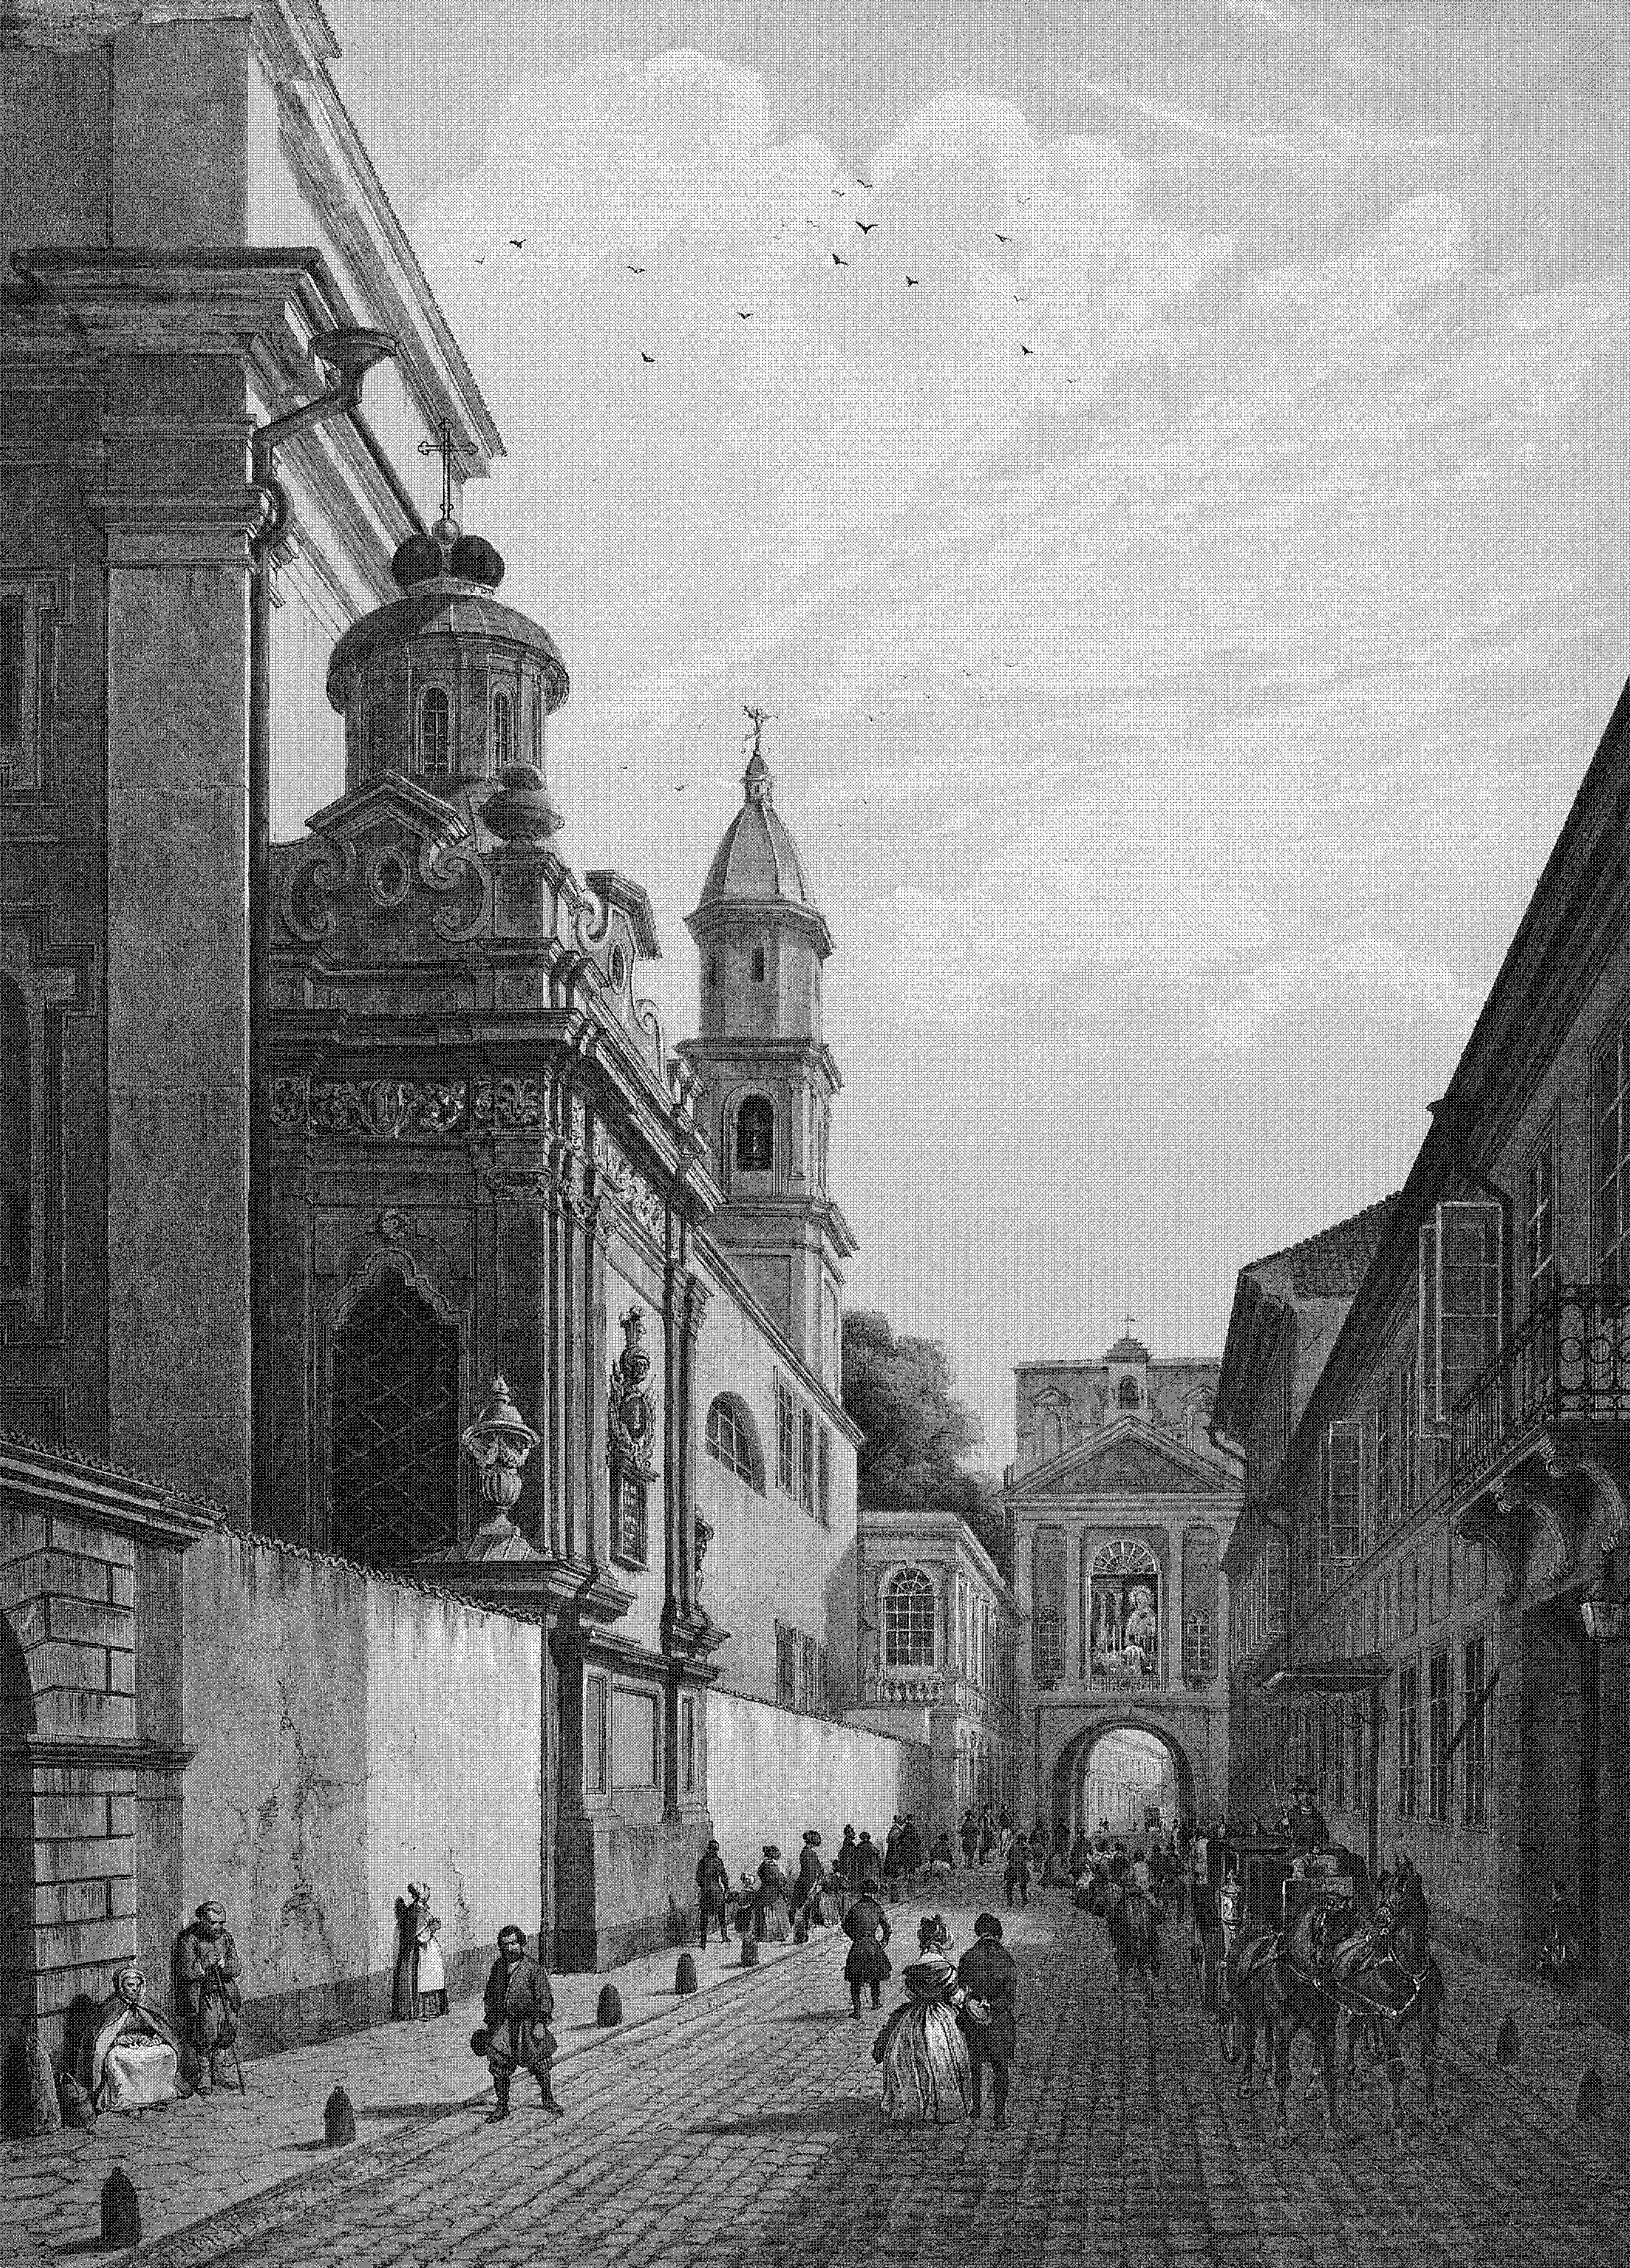
\includegraphics[width=\textwidth]{ilustra-02.png}
    \caption{Ostra Brama, em polonês ``Portão do Alvorecer'', Vilna, 1846.}
\end{figure}

No que toca às suas características naturais, a Lituânia, também, muito
difere do Brasil. A localização do país é limitada pelos paralelos 54 e
56 Norte, o que o situa mais do que a meio caminho entre o Equador e o
Polo Norte. Caso se localizasse nas coordenadas correspondentes no
hemisfério sul, o país acabaria nas águas gélidas e nevoentas do Canal
de Beagle, que separa a ilha da Terra do Fogo da Patagônia continental.
Profissionais da meteorologia descrevem a Lituânia como detentora de um
sub"-tipo mais frio do clima continental úmido, o que nada significa até
que se vivenciem os longos, escuros, úmidos e gélidos invernos do país.
Esse também é o tipo de clima atribuído à zona meridional dos Andes
argentinos. 

Embora os verões se escaldem na luz do sol e cores
brilhantes, seu efeito sobre a paisagem é de uma duração embaraçosamente
curta. As primaveras são deliciosas, mas elas também vêm e vão
apressadas. O início do outono, com a dramática mudança de cor das
folhagens, pode ser divino; mas é mais acaso que regra. Os habitantes
locais apreciam os curtos porém quentes dias do outono, porque trazem
consigo os frutos da floresta, como por exemplo uma grande variedade de
cogumelos comestíveis. A neve pode tornar os invernos cinzentos menos
imperdoáveis, embora possa assumir um caráter bem desagradável. De
qualquer modo, em qualquer época do ano, a floresta lituana é uma
maravilha por si só. Pode"-se ``passear horas a fio sem fatigar a
vista,'' como explica Czesław Miłosz, escritor polonês nascido na
Lituânia e ganhador do prêmio Nobel, ``pois, como as cidades humanas, as
três colônias têm o seu próprio caráter --- formando ilhas, zonas e
arquipélagos\ldots{}'' que, combinados aos inúmeros riachos, rios, lagos
e pântanos, induzem uma sensação de intimidade que decididamente tempera
``a severidade do norte.''\footnote{Czesław Miłosz, \textit{The Issa
  Valley}, trad. Louis Iribarne. Nova York: Farrar, Strauss and
  Giroux, 1978, p. 3.} Pois, em sua maior parte, a Lituânia pode ser
descrita como um oceano de árvores, e considerada a rainha das florestas
verde"-escuras, nas palavras de um poeta russo, embora o nome do país
sabidamente venha da palavra lituana que significa chuva ou jorro. Seja
como for, tudo aquilo abunda na Lituânia.

Essa fusão de água e madeira torna a Lituânia elusiva, difícil de
abarcar e fácil de inundar. Por conseguinte, o país é comparável a uma
serpente que se esgueira com facilidade da terra para a água; uma
criatura silvestre que não obstante foi sempre bem"-vinda nos lares dos
lituanos pagãos. A palavra lituana para cobra tem a mesma raiz da
palavra que denota vida, dando uma ideia do papel vital da cobra na
mitologia local. Segundo os missionários jesuítas enviados à Lituânia no
século \textsc{xvi}, a serpente naquele então ainda era venerada pelos
habitantes locais, que seguiam as tradições de seus ancestrais pagãos.
Os jesuítas que chegaram à Lituânia a convite do grão"-duque para fazer
prevalecer a fé católica acabaram instilando um caráter barroco ao país.
Como resultado, a Lituânia parece um primo distante do Brasil,
comungando de um vocabulário estético similar de expressão religiosa.

Como no Brasil, o barroco na Lituânia durou muito mais do que em outras
regiões, tornando"-se, por assim dizer, o estilo inato do país. A madeira
é largamente utilizada no barroco lituano, de modo que os ornamentos e
esculturas em madeira de Aleijadinho, por exemplo, não pareceriam
deslocados em muitas das igrejas católicas da Lituânia. Aqui e ali,
ademais, Vilna também, devido a seu barroco local instituído pelos
jesuítas, comunga da afinidade visual de Salvador da Bahia. As duas
cidades são colinosas, o que em ambos os casos faz da arquitetura
barroca local menos espalhada e mais ondulosa. Em se tratando de
jesuítas, cabe sublinhar que eles abordaram suas missões em ambos os
países com um objetivo semelhante em mente: fazer os nativos abraçar a
doutrina católica. Pregar nos idiomas locais era instrumental para a
redenção das almas. Assim, ao passo que os missionários, no Brasil,
aprendiam o tupi e outras línguas nativas para nelas evangelizar, um
padre português de Coimbra, Emanuel de Vega, em torno de 1580 chegou a
Vilna para dar aulas no colégio jesuíta local e aprender a pregar em
lituano, um dos primeiros casos de que se tem notícia no Grão"-Ducado da
Lituânia.

\section*{\textit{Pasiilgau}, \textit{nostalgia}, \textit{ilgesys}}

Sem dúvida, um dos laços mais vigorosos das relações entre o Brasil e a
Lituânia se deve à imigração --- sobretudo de lituanos, mas também de
judeus e poloneses --- para o Brasil a partir da região que historicamente
tem sido associada ao Grão"-Ducado. Ao que tudo indica, ela começou
tímida no fim do século \textsc{xix}, atingindo o pico na década de 1920,
com dezenas de milhares de novas chegadas. No bairro paulistano de Vila
Zelina, há ainda bastante evidência da presença lituana no Brasil; e
marcas da cultura \textit{litvak} podem ser identificadas na grande comunidade
judaica brasileira. Apesar disso, depois de um século de assimilação,
perdeu"-se de vista a Lituânia no Brasil. Ademais, assim como costuma
ocorrer com a maior parte das histórias de migração, esse movimento de
pessoas criou uma associação parcial entre os países; enquanto a memória
da Lituânia permaneceu esporádica no Brasil, na Lituânia, o Brasil é
raramente visto como tendo algo a ver com com a história da nação.

A fim de capturar melhor essa parca conexão, perguntei a brasileiros de
origem lituana sobre o significado da saudade. Duas irmãs --- Mafalda e
Rute --- que nasceram em São Paulo numa família lituano"-ucraniana, mas que
foram mais tarde levadas para Vilna por seus pais, na esperança de uma
vida melhor na Lituânia soviética, contaram suas estórias de imigrantes
em ambos os países. Seu pai imigrou para o Brasil na década de 1920 e,
quando a família retornou à Lituânia em 1960, Mafalda tinha 15 anos e
Rute, 9 (havia também um irmão mais velho, que mais tarde retornou ao
Brasil). Embora recebidos com certos privilégios como uma ``família
lituana'' repatriada pelas autoridades soviéticas, a língua materna dos
três filhos permaneceu o português. 

O sistema comunista lituano
baseava"-se menos na cultura e no idioma de etnia local do que na
ideologia do internacionalismo proletário, escorado na supremacia da
abrangência russa. Manter laços com o Brasil e falar uma língua
estrangeira, contudo, significava fazer parte de uma lista de proscritos
políticos; mas nem se permitia que a família como um todo retornasse ao
Brasil. Assim, eles viveram suas vidas em Vilna em plena contradição:
eram vistos como lituanos natos, porém não tão natos em termos de
solidariedade linguística e educação ideológica --- intrusos no ninho.

Enquanto Mafalda (um nome excêntrico na Lituânia) permaneceu no país, 
Rute (variação de um nome lituano muito comum), depois de
dezessete anos na Lituânia, recebeu permissão para deixar a União
Soviética e retornou ao Brasil. Do ponto de vista político, as coisas
mudaram tão logo a Lituânia conquistou a independência em 1990, embora a
definição limitadora do significado de ser lituano houvesse se
cristalizado. Assim, malgrado os diferentes padrões migratórios, ambas
as irmãs se sentiam deslocadas em suas duas pátrias. Mafalda mora em Vilna, mas
``considero"-me primeiramente brasileira, depois lituana. Por
mais que eu queira, não posso esquecer o Brasil, pois basta dizer o meu
nome na Lituânia, e inevitavelmente tenho que explicar de onde vem esse
nome, pois ninguém nunca ouviu um nome igual aqui. Além disso, toda a
minha vida está muito ligada ao Brasil. Minha irmã vive lá, meu falecido
irmão viveu lá, seus filhos também vivem lá, minha filha representa a
Lituânia no Brasil, lá ficaram meus amigos de infância. Eu até durmo de
acordo com o horário do Brasil, tenho dificuldades em levantar"-me cedo,
pois no Brasil ainda é noite.''

Por outro lado, Rute hoje mora no Estado de São Paulo, mas ``amo a Lituânia pela sua história, suas conquistas,
seu passado (fiquei sabendo dele através dos contos de meus pais), e
também porque morei neste lindo país. Aqui viveram meus tios, aqui eles
lutaram contra os inimigos, os ocupantes. Amo a Lituânia pois tenho
sangue lituano. Basta pensar nisto e meus olhos se enchem de lágrimas.
Eu sei que faço parte deste país, minhas raízes estão na Lituânia. Não
posso dizer o mesmo do Brasil. Apesar de ter nascido aqui, não sinto o
mesmo amor, os sentimentos tão profundos que nutro pela Lituânia. No
Brasil está a minha família, meus netos, eu vivo aqui e aqui ganho o meu
dinheirinho para sobreviver, a minha pensão. Apesar disto, aqui
sinto"-me uma estrangeira. Na Lituânia deixei meus pais, minhas memórias,
a cultura lituana que tanto me encantou.''

De qualquer maneira, conhecer intimamente a Lituânia modificou a perspectiva 
dela sobre seu lugar de nascimento. ``O fato de ter vivido no Brasil e também na Lituânia deu"-me
uma experiência muito positiva, me enriqueceu, fez"-me ver que cada país
tem o seu modo de viver. Isso deu"-me forças para seguir vivendo.'' Para
Mafalda, o mesmo poderia ser dito sobre sua relação com a Lituânia,
distorcida por seu amor pela terra natal. ``Talvez o primeiro ar que
respirei, foi o ar do Brasil. Talvez porque as escolas que frequentei
sendo criança me ensinaram a amar e respeitar a pátria, e minha pátria
era o Brasil na época. Eu não tenho sangue brasileiro no corpo, mas meu
espírito é brasileiro, sem dúvida.''\footnote{Entrevista realizada pelo autor, 5 de setembro de 2020.}

Contemplar o oceano na direção da lembrança do Brasil a partir da
perspectiva de toda uma vida passada na Lituânia exige as palavras
certas. ``Saudade para mim tem muitos significados, por isso é difícil
traduzir essa palavra. Em lituano nós apenas constatamos um fato, quando
dizemos que \textit{pasiilgau}, ou `tenho saudades'. Já em português nesta
palavra há muito mais sentimento, memórias, imagens, amor, e é por
isso que ao pronunciá"-la sorrimos através de lágrimas --- sorrimos,
porque nos trazem memórias muito agradáveis, e lágrimas porque se trata
de um passado irreversível. Em lituano, as palavras
\textit{nostalgia}, \textit{ilgesys}, lembram mais um sentimento
físico, uma dor. A saudade designa o desejo de algo bom, positivo, mas
geralmente que já não existe, a vontade de ter de novo, de voltar trás.
Gosto da explicação --- saudade é quando nossa alma diz que quer voltar
para um lugar que você ama, mas este lugar não existe mais.''

Ao mesmo
tempo, avistar a memória da Lituânia a partir do Brasil é espantosamente
mais imediato e cheio de detalhes, exprimindo a sensação de se estar em
contato total com um mundo que há décadas permaneceu geograficamente
fora de alcance. ``Tenho saudades dos meus parentes queridos: primos,
tios, tias, da vida rural, do inverno, da neve, de patinar no gelo, de
andar de trenó, de rolar na neve, das estações do ano, sobretudo da
primavera com suas violetas, lírios do vale, de ver as árvores brotarem
depois de uma boa chuva primaveril, macieiras em flor; de veranear na
casa de meus tios, trabalhar nos campos, cortar a grama para que os
animais tenham seu feno, sem falar no outono com seus cogumelos, suas
árvores com folhas de cores diferentes do amarelo clarinho ao marrom
escuro, desenhos de inverno nas janelas, pinheirinhos nevados, bonecos
de neve com nariz de cenoura... Há tempo que não vejo tudo isto. Tenho
saudades.''\footnote{Entrevista realizada pelo autor, 5 de setembro de
  2020.}

\section*{Um conto de amor radical pela terra natal}

Deve ter sido essa imagem perfeita e tangível da Lituânia que incitou a
imaginação do jovem Joaquim Maria Machado de Assis a ponto de se sentir
atraído pela Polônia. Machado jamais pôs os pés na Lituânia (nesse caso,
nem na Polônia ou na Europa), e é pouco provável que tenha alguma vez
encontrado alguém da Lituânia; teria sido igualmente improvável ele
descobrir algo sobre o país nas livrarias ou bibliotecas do Rio de
Janeiro. Contudo, no início de sua carreira de escritor, ao menos por
alguns raros momentos, o espírito errante e incansável do país dominou a
sua mente suscetível. Segundo seu próprio testemunho, aquela terra
distante havia atravessado o oceano para chegar até ele por meio de uma
tradução francesa. 

Por conta disso, a Lituânia não foi nomeada, mas se
apresentou sob a pele de outra nação. Assim, a Lituânia deslizou até o
alcance de Machado e, por extensão, do Brasil, de maneira imperceptível,
como uma confusão cartográfica. Isso se deveu em parte ao fato de que,
naquela altura, uma boa parte da Lituânia fosse percebida como
pertencente ao passado. Por razões geopolíticas, o Grão"-Ducado da
Lituânia desaparecera do mapa da Europa no início do século \textsc{xix} e,
com ele, impôs"-se a ideia, amplamente aceita, de que o país fosse mais
nostálgico que real. Na opinião do mais famoso poeta nacional, Adam
Mickiewicz, graças a seu passado glorioso e seu presente irrealizado, a
Lituânia não passa de um feliz tema para se fazer poesia. Na verdade, a
Lituânia estava pronta para a saudade --- sentimento romântico que negocia
intimidade por publicidade.

O volume de poemas escrito por Machado e intitulado \textit{Crisálidas},
publicado em 1864 no Rio de Janeiro, contém dois poemas baseados no tema
da Lituânia. Em ambos os casos, o país se apresenta num finíssimo
disfarce sob os títulos de \textit{Polônia} e \textit{Alpujarra}.
Casualmente, aquele ano marca um divisor de águas na história da
Lituânia, pois é o momento em que se inicia a compreensão moderna do
país mais como território delimitado pela aplicação dos princípios de
singularidade étnica e uniformidade linguística do que como terra
erguida em torno da heterogeneidade cultural da região. 

Ao longo do
tempo, esse tipo de pensamento tornou a Lituânia menor e mais estreita,
como também jogou fora boa parte de seu passado. Os poemas de Machado
são reflexões de seu fascínio pelas imagens e a estória de vida de
Mickiewicz, que nasceu em 1798 numa família de fala polonesa, numa
região da Lituânia que hoje se situa na Bielorrússia. Essencialmente,
Mickiewicz fez parte de uma Lituânia que, na época em que Machado
criativamente tentava apreendê"-la, já deixara de existir. Por outro
lado, aquela Lituânia de outrora trouxe fama a Mickiewicz, pois ela lhe
permitiu desabrochar como um verdadeiro romântico, ou seja, tornar"-se
alguém que se sente sempre deslocado tanto no tempo como no espaço.
Machado dedicou \textit{Polônia} a Mickiewicz, e \textit{Alpujarra} é a
tradução de uma balada de Mickiewicz retirada de seu conto histórico
\textit{Konrad Wallenrod}. Esse longo poema descreve as lutas dos lituanos
pagãos contra os cruzados na Idade Média. É um enredo complexo, mas a
ideia principal do episódio de Alpujarra é a de conferir à luta lituana
um contraponto na história europeia. Nesse caso, foi a luta dos mouros
de Granada contra os castelhanos cristãos. Em suma, \textit{Alpujarra} é
uma balada da reconquista, mas, situando"-a num cenário lituano pagão,
Mickiewicz a transformou num conto de amor radical pela terra natal.

Mickiewicz cresceu às margens do rio mais importante da Lituânia,
chamado Nemunas em lituano, mas também Niemen em polonês. De acordo com
certos relatos, os antigos gregos e romanos equalizavam o rio a Cronos
ou Saturno, deus do tempo que devorou os filhos a fim de comprovar a
força destrutiva do passado sobre o futuro. Para os geógrafos da era
clássica do Mediterrâneo, tais como Heródoto e Ptolomeu, o rio Cronos
conferia ideia física à extensão do conhecimento humano.

Para além do curso d'água, ficava uma região congelada no tempo. De
maneira que o território hoje ocupado pela Lituânia era compreendido
como uma esfera existente fora da narrativa e, portanto, além da
possibilidade de ser imaginada e descrita; não muito diferente de como o
interior do Brasil foi compreendido pelos europeus à época dos
descobrimentos. De todo modo, do ponto de vista geográfico, o Niemen
jamais foi um rio polonês, pois nenhum trecho dele passa pela Polônia.
Foi sobretudo por intermédio da poesia de Mickiewicz que o rio ganhou
ressonância no espírito polonês. Por outro lado, o nome Nemunas é
utilizado por lituanos ao redor do mundo para afirmar sua afeição e
lealdade ao país. Em São Paulo, por exemplo, um grupo de danças
folclóricas lituanas se chama \textit{Nemunas} e um outro,
\textit{Rambynas}, monte sagrado às margens daquele rio.

Mickiewicz cursou a universidade em Vilna e passou a maior parte de sua
juventude na Lituânia. Embora se considerasse lituano de nascença, ele
escreveu exclusivamente em polonês. Aos vinte e cinco anos de idade, por
pertencer a sociedades estudantis nativistas patrióticas, o poeta foi
banido para sempre da Lituânia pelas autoridades russas tzaristas. Com
essa perda (pessoal) do país natal, ele partiu para o exílio,
estabelecendo"-se finalmente em Paris, onde se tornou o mais famoso dos
românticos europeus. Na França, o bardo polonês percebeu ser menos
escritor do que peregrino, promovendo a própria imagem como uma espécie
de cabalista ou profeta. Ele sentia saudade da Lituânia; mas via na
ressurreição política da Polônia crucificada o futuro da Europa. Em
harmonia com esse sentimento, em 1855 o poeta"-peregrino morreu em
Constantinopla enquanto tentava organizar uma legião polonesa durante a
Guerra da Crimeia. A maior parte da obra do poeta foi inicialmente
traduzida do polonês para o francês, situando"-o junto a autores
franceses do período.

Muito da mística poética e da fama romântica de Mickiewicz se deve a seu
vínculo com a (antiga) Lituânia, embora defendesse ao mesmo tempo o
renascimento da Polônia. Ademais, suspeita"-se que a mãe de Mickiewicz
tivesse origens judaicas. Em sua mente, essa unidade herdada composta
por duas dissonâncias --- um corpo extinto e uma alma revolucionária, a
velha Lituânia e a nova Polônia --- fazia dele um emissário de verdades
universais. Mesmo assim, em seus poemas, Mickiewicz era quase sempre
extremamente local, ou seja, acentuadamente lituano. Quase imediatamente
após ser forçado a deixar a Lituânia, ele escreveu um poema dedicado ao
rio de sua infância, que de certa forma se tornara a imagem central da
paisagem nativa que configurou grande parte de sua obra criada no
exílio. O poema começa como um hino: ``Niemen, meu rio nativo! Onde
estão aquelas águas/\,Para as quais nos arremessávamos por campinas
floridas/\,E que coletávamos com nossas mãos juvenis/\,Para beber ou
imergir nossas faces ardentes?'' Poucas estâncias depois, porém, ele
termina abruptamente numa elegia: ``Onde a doce angústia que a idade
arrebatada traz?\ldots{} Tudo se foi, mas por que não minhas
lágrimas?''\footnote{Adam Mickiewicz, ``Do Niemen'', trad. para o
  inglês de Adam Mickiewicz, \textit{The Sun of Liberty. Bicentenary
  Anthology 1798--1998}. Edição bilíngüe polonês"-inglês. Varsóvia:
  Energia, 1998.}

Machado se deixou claramente emocionar pela imagem e pelo sentimento
evocados pelo tema do rio no poema de Mickiewicz. O Niemen era ao mesmo
tempo concreto e eterno, particular e universal, fazendo o tempo fluir e
modelando a memória. Machado compôs \textit{Polônia} como homenagem à
nação polonesa batalhadora, mas também como alguém que tinha vivenciado
uma perda pessoal. O escritor dedicou \textit{Crisálidas} a seu pai que
havia recentemente falecido. A sensação do poema é a de um incalculável
sentido de passagem do tempo que torna a memória íntima em algo doloroso
porém suave. Essa abordagem pessoal do tema da história (estrangeira)
alça \textit{Polônia} desde a condição de cantilena para símbolo da
lembrança. Machado ecoa o bardo polonês, mas apenas de maneira evasiva,
como se não tivesse certeza de captar corretamente a imagem da Lituânia.
Afinal de contas, ele leu Mickiewicz em francês, imerso no ambiente
tropical brasileiro, longe da Europa, e ainda mais longe da Polônia. Sua
percepção nebulosa da Lituânia se baseava numa tradução estrangeira da
transfiguração polonesa do país. Assim sendo, o poeta brasileiro se
detém em nomear coisas canonizadas por Mickiewicz.

\begin{verse}
Eras livre, --- tão livre como as águas \\
Do teu formoso, celebrado rio;\\
A coroa dos tempos\\
Cingia"-te a cabeça veneranda;
\end{verse}

Além disso, Machado torna mais clara sua leitura sugestiva da paisagem
ribeirinha nativa de Mickiewicz ao incluir uma nota no fim do poema: ``O
rio a que aludem os versos é o Niemen. É um dos rios mais cantados pelos
poetas polacos. Há um soneto de Mickiewicz ao Niemen, que me agradou
muito, apesar da prosa francesa em que o li, e do qual escreve um
crítico polaco: ``Há nesta página uma cantilena a que não resiste nenhum
ouvido eslavo {[}\ldots{}{]} Assim consagrado, o soneto de Niemen correu
toda a Polônia, e só deixará de viver quando deixarem de correr as águas
daquele rio.''\footnote{Machado de Assis, \textit{Crisálidas}. Rio de Janeiro: Garnier, 1864.} Depois de apontar primeiro para o Niemen,
Machado rapidamente se volta para o reino celestial da Lituânia. Dessa
vez ele é mais eloquente, embora permaneça cauteloso, como se temesse
adentrar em águas ignotas. Apesar da hesitação, a terra desconhecida
cintila.

\begin{verse}
E a desvelada mãe, a irmã cuidosa,\\
A santa liberdade,\\
Como junto de um berço precioso,\\
À porta dos teus lares vigiava.\footnote{Machado de Assis, ``Polônia'', ibid.}
\end{verse}

Embora ausente das notas de Machado, a visão da ``desvelada mãe'' evoca
a imagem do ícone sagrado da Virgem que adorna e protege Vilna. A
capital lituana se localiza às margens do principal tributário do
Nemunas, o rio Neris. Também conhecido em polonês e iídiche como Viliya
--- haja vista à epígrafe de Sutzkever: ``Como sinais cabalistas, douram
as bordas/\,Onde seus abetos farfalham nas margens do Viliya.'' O ícone
folheado a prata está colocado numa capela acima de um dos portões da
cidade. Em polonês, essa entrada é conhecida como \textit{Ostra Brama}, ou
Portão Pontudo. Em lituano moderno, ela é chamada de \textit{Aušros
Vartai} --- Portão do Alvorecer. Para Mickiewicz, o rosto terno da Virgem
melancólica no portão sintetiza a essência da Lituânia tanto como
promessa como reparo: uma oferta votiva e uma metamorfose unidas por sua
peregrinação no exílio. 

A estátua de Mickiewicz enfeita uma das praças
do centro antigo de Vilna; e o portão assoma com freqüência ao longo
deste livro, lembrete sutil de que nenhum conto local ou relato
estrangeiro pode deixá"-lo de lado. No universo de Vilna, essa imagem
sagrada é o fragmento de âmbar da cidade --- ele reluz à claridade da
lírica de Machado. O poeta deixa porém entreaberta a visão da cidade,
como se aguardando que a Vilna anônima e invisível se torne mais íntima
e confidencial. \textit{À porta dos teus lares vigiava.} Espero que o
livro siga o exemplo, iluminando desta feita Vilna inteira na língua
materna de Machado.